\documentclass[a0,final]{a0poster}
%%%Load packages
\usepackage{multicol} 			%3-column layout
\usepackage[left=2cm,right=2cm,bottom=0cm,top=0cm]{geometry}			%Reset margins
\usepackage{mathpazo}			%Load palatino font & pazo math
\usepackage{color}				%Needed for colour boxes & coloured text
\usepackage{amsmath}

\usepackage{graphicx}     		%Needed to import images

\usepackage[]{algorithm2e}



\DeclareGraphicsExtensions{.pdf,.png,.jpg}

\graphicspath{ {./images/} }




%%%Define colours and lengths
\definecolor{headingcol}{rgb}{1,1,1}			%Colour of main title
\definecolor{boxcol}{rgb}{0.7,0.2,0.2}		%Edge-colour of box and top banner
\fboxsep=1cm							%Padding between box and text
\setlength{\columnsep}{2cm}				%Set spacing between columns

%%%Format title
\makeatletter							%Needed to include code in main file
\renewcommand\@maketitle{%
\null									%Sets position marker
{
\color{headingcol}\sffamily\VERYHuge		%Set title font and colour
\@title \par}%
\vskip 0.6em%
{
\color{white}\sffamily\large				%Set author font and colour
\lineskip .5em%
\begin{tabular}[t]{l}%
\@author
\end{tabular}\par}%
\vskip 1cm
\par
}
\makeatother

\title{BA Scale Free Networks}

\author{Dalwinder Bagdi, Tanvi Bhardwaj, Ankeet Dhanji, Dani Grayston, Alexandru Stoenescu \& Shuai Wang (Robert)\\
University of Manchester - Group 5}

\begin{document}

\hspace{-3cm}								%Align with edge of page, not margin
\colorbox{boxcol}{							%Coloured banner across top
\begin{minipage}{1189mm}					%Minipage for title contents
\maketitle
\end{minipage}}
\vspace{1cm}

\begin{multicols}{3}							%Use 3-column layout
\raggedcolumns							%Don't stretch contents vertically

%%%Column1
\section*{Introduction}
This is an introduction

\section*{Algorithms}




\begin{algorithm}[H]
 \KwData{Total number of nodes to be added T; \\
       Initial number of nodes $n_0$; \\
       Minimum degree M.\\}
 \KwResult{scale-free multigraph G}
Add $n_0$ nodes to G.\\
%Connect every node in G to every other node in G, i.e. create a complete graph. \\
t = 0
 \While{!t$<$T}{
    Create a new node i.\\

 \While{!m$<$M}{
Pick a node j at random from the graph G with probability of each node as P[j].\\
Pick a real number R uniformly at random between 0 and 1.\\
     \If{P[j] $>$ R}{
        add j to i's adjacency list\\
 	m++
    }
Add i to the adjacency list of each node in its adjacency list.\\
Add i to to the graph.\\
}
$ P[i] = \frac{k_i}{\sum\limits_{k=1}^N} k_j$, N = $n_0$ + t -1\\
t++
    }
return graph G\\
 \caption{BA Network Generation Algorithm}
\end{algorithm}



\columnbreak

%%%Column 2



\section*{Algorithm in Action}
Below is an illustration of the BA algorithm being applied to a small network.
It initially starts of with two nodes that are connected to each other. After adding more nodes, a few individual nodes start to gain more connects than the others.\\
\centerline{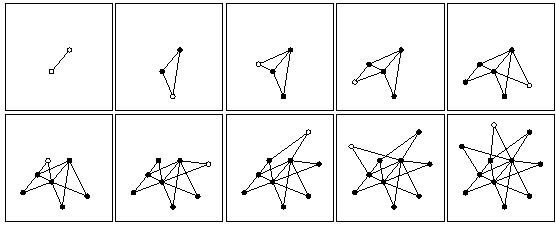
\includegraphics[width=30cm]{growth.jpg}}

\section*{Examples of Scale Free Networks}

There are many various examples of Scale Free Networks. These range from Air Traffic Networks to the Internet. Below is an example of a Scale Free network that was generated by the BA algorithm.
\newline
{\centering
\centerline{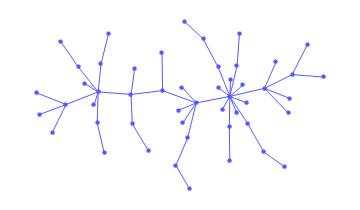
\includegraphics[scale=1.5]{BA.jpg}}}
\newline
The BA network above is created using 50 nodes that each initially had a degree of 1.
After applying the BA algorithm, it is visible there are very few nodes with a high degree. This is due to nodes that have a higher degree have a high probability of gaining more links, thus the "rich" are becoming "richer". This also means that the new network created follows Power Law distribution.
\newline

\centerline{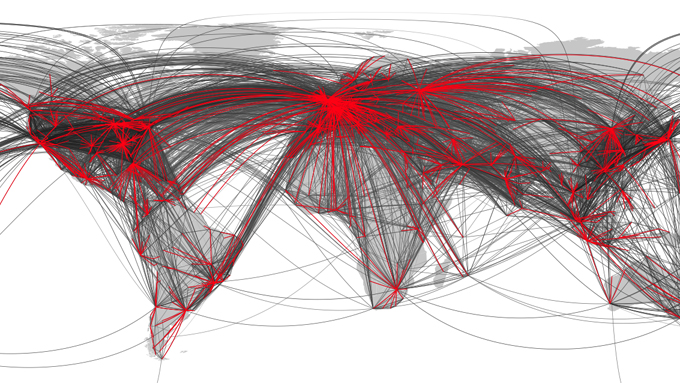
\includegraphics[width=35cm]{airtraffic.jpg}}

The figure above shows the Global Air Traffic Network. It shows the there are a few internation airports (nodes) in the world that connect (link) to many different places. However most airports only connect to a small number of places, thus these airports have a small degree. Again this Air Traffic Network has the Power Law Distribution property.


\columnbreak

%%%Column 3


\section*{Analysis}
\subsection{Parameters}
There are three parameters in this algorithm. They are the totoal number of nodes T;  Initial number of nodes $n_0$ and the minimum degree M. \\
\begin{description} 
  \item[Initial number of nodes $n_0$] should be a small number. It is the number of nodes a graph start with.
  \item[Total number of nodes to be added T] is the total timestep. Increasing T will add more nodes to the network, making it more dense. The nodes that have a high degree will continue to grow rapidly (in terms of links) and the nodes with less degree will not gain as many links.
  \item[Minimum degree M] is the minimum number of links the new node starts with. It will be linked M times to existing nodes according to their probability of being linked. If M is large then the new node is more likely to gain extra connections in subsequent iterations of the algorithm, otherwise not.
\end{description}

\section*{Structual and Topological Properties}

\begin{description} 
\item[Small World] Small-world network is a network that every two nodes in the network has at least one path. i.e. most nodes can be reached from every other nodes by a small number of steps. 
  \item[Power Law Distribution] The connectivity of BA scale free network has the property of Non-homogeneity: very few nodes have many links but most nodes have very few links.
  \item[Preferential Attachment] The probability of a new node getting connected with a node i is: $P[i] = \frac{k_i}{\sum\limits_{k=1}^N} k_j$ (see the algorithms part)


  \item[Scale Free] The degree distribution should follow $P(k) \sim k^{-r}$, where r is between 2 and 3 usually.
\item[Average Path Length] The average path length (L) is smaller in a BA network than in a random graph for any N. The existence of hub nodes makes L << N, in accordance with the small world property. L increases approximately logarithmically with N. It follows the given formula :  $\frac{\ln{N}}{\ln{\ln{N}}}$

\item[Clustering Coefficient] The clustering coefficient, also called network density, is a measure of the tendency of nodes to form cliques in a given network. The clustering coefficient of a scale-free network is much higher than that of random networks of the same size, and this difference slowly increases with the number of nodes. The density of the clusters increases with an increase in the value of the coefficient.

\item[Connectivity] Since a BA network model follows a power law distribution, a few nodes have many links and act as hubs whereas most of the nodes have very few links. This heterogenous nature allows the network to be robust against random removal of nodes, thereby not affecting the connectivity hugely.

\end{description}

\section*{Similarities between the networks and real-world networks}
The scale-free nature of real networks is rooted in two generic mechanisms shared by many real networks. First, most real- world networks describe open systems that start from a small nucleus and grow by the continuous addition of new nodes throughout the lifetime of the network. For example, the World Wide Web grows exponentially in time by the addition of new web pages.
			
Second, most real networks exhibit preferential attachment, such that the likelihood of connecting to a node depends on the node’s degree. For example, a web page will more likely include hyperlinks to popular documents with high degrees, because highly connected documents are easy to find. 




\section*{Conclusion}
In this poster, a Scale Free BA network was defined, An algorithm was presented. Several parameters were introduced. The results were analysed as these parameters vary. The difference as the size increase and similarities were investigated and topological properties were addressed. In addition, comparison with small real-world networks was provided. 
%\nocite*

\bibliographystyle{plain}
\begin{bibliography}{6}

\bibitem{1} Scale free network. http://www3.nd.edu/~networks/Linked/fig7_1.jpg [Accesed May 2014]
\bibitem{2} Air traffic network of world: http://www.mccormick.northwestern.edu/images/gallery/June%2012/brockmannbanner2.jpg [Accesed May 2014]
\bibitem{3} Network generated using the BA algorithm. http://upload.wikimedia.org/wikipedia/commons/2/2e/Barabasi_Albert_generated_network.jpg [Accesed May 2014]
\bibitem{4} Co-stardom network. http://en.wikipedia.org/wiki/Co-stardom_network [Accesed May 2014]
\bibitem{5} Internet. http://en.wikipedia.org/wiki/Internet [Accesed May 2014]
\bibitem{6} World Wide Web. http://en.wikipedia.org/wiki/File:WorldWideWebAroundWikipedia.png [Accesed May 2014]

\end{bibliography}

\end{multicols}
\end{document}
